%%=============================================================================
%% Proof-of-concept: Conventioneel
%%=============================================================================

\chapter{\IfLanguageName{dutch}{Proof-of-concept: Conventioneel}{Proof-of-concept: Conventional}}%
\label{ch:proofofconceptConventioneel}

\section{Inleiding}

In dit hoofdstuk zal een overzicht gegeven worden over hoe de conventionele webshop is opgebouwd. Hier zal echter niet dieper ingaan op het technische aspect van de React componenten of de API-calls die gerealiseerd zijn.

\section{Mock-ups}

Alvorens er een lijn code geschreven wordt zijn er mock-ups gemaakt voor de mobiele versie \ref{fig:mobileMockUps} en de desktop versie, beide voor de Home Pagina \ref{fig:desktopHomeMockUp} en de Detail Pagina \ref{fig:desktopDetailMockUp}. Zoals eerder vermeld dienen de mock-ups als een basis voor de conventionele versie van de webshop om een goede UX/UI te voorzien.

\begin{figure}
	\centering
	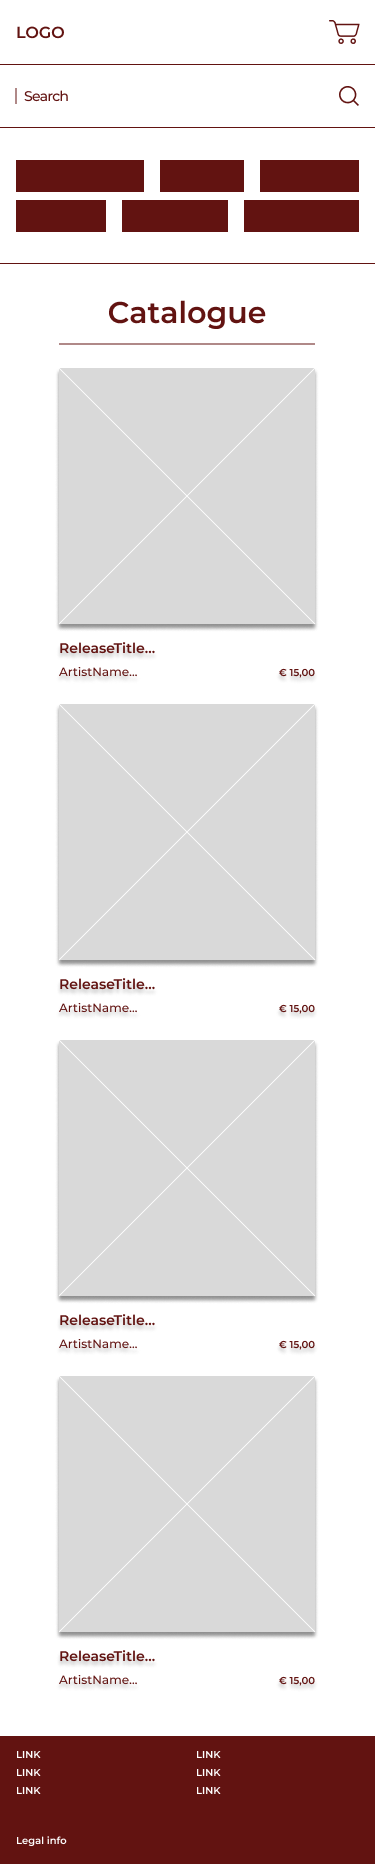
\includegraphics[width=0.3\linewidth]{graphics/HomePageMobile}
	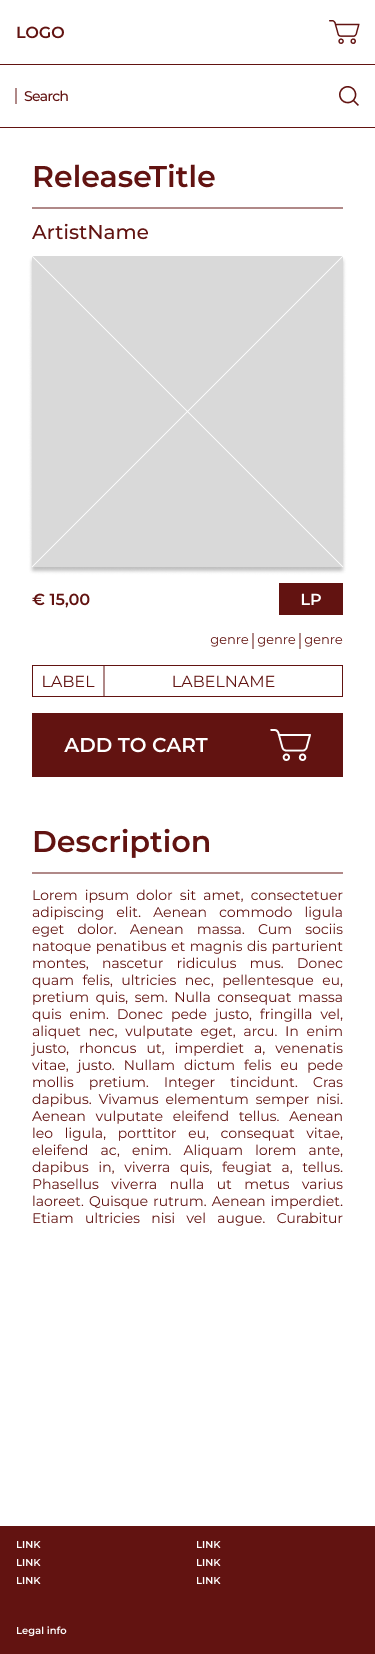
\includegraphics[width=0.3\linewidth]{graphics/DetailsPageMobile}
	\caption[Mock-Ups Mobile]{Mock-Ups Mobile}
	\label{fig:mobileMockUps}
\end{figure}

\begin{figure}
	\centering
	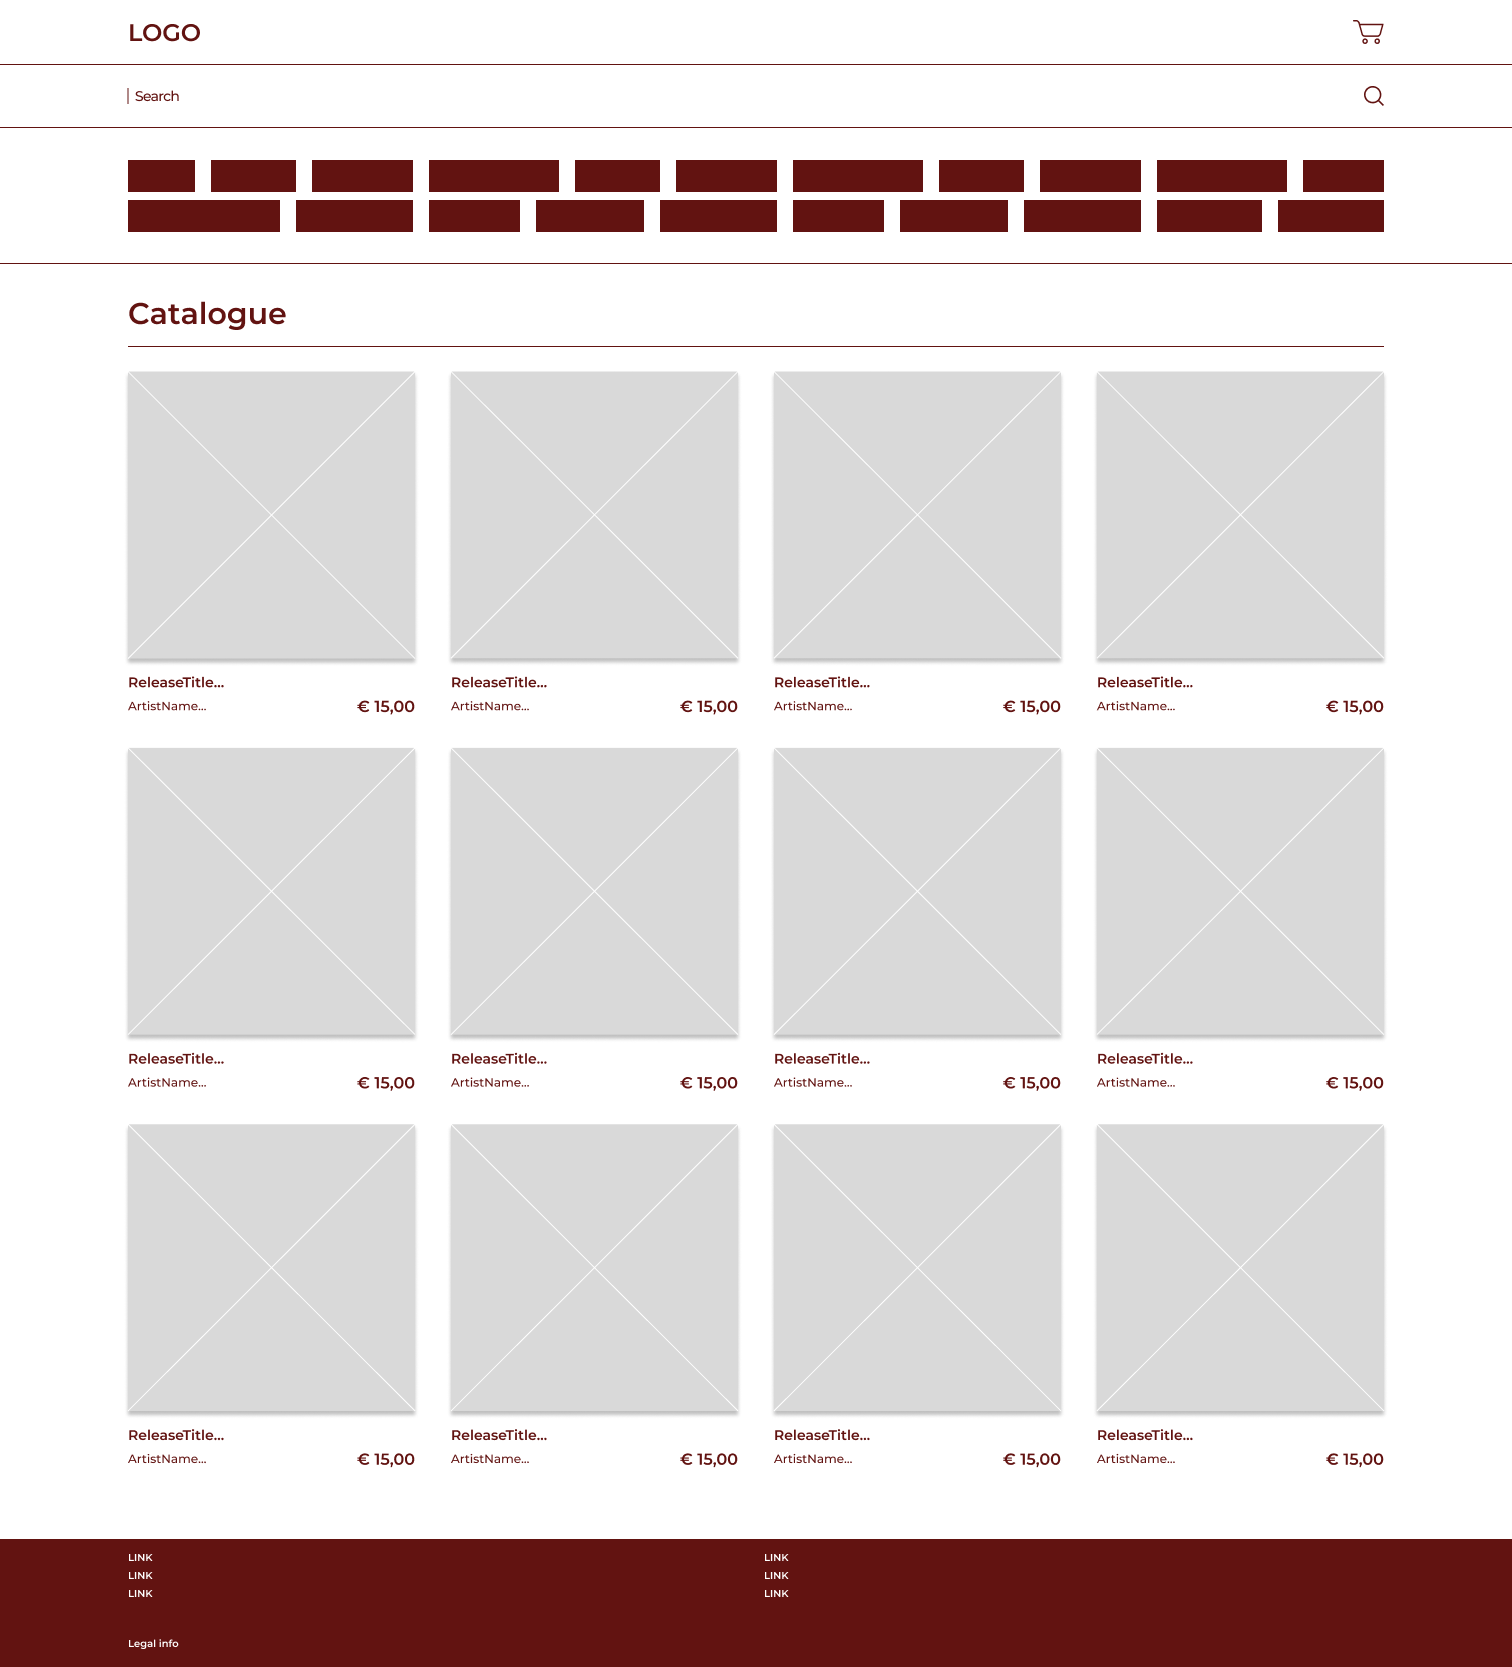
\includegraphics[width=1\linewidth]{graphics/HomePageDesktop}
	\caption[Mock-Up Desktop]{Mock-Up Desktop Home Pagina}
	\label{fig:desktopHomeMockUp}
\end{figure}

\begin{figure}
	\centering
	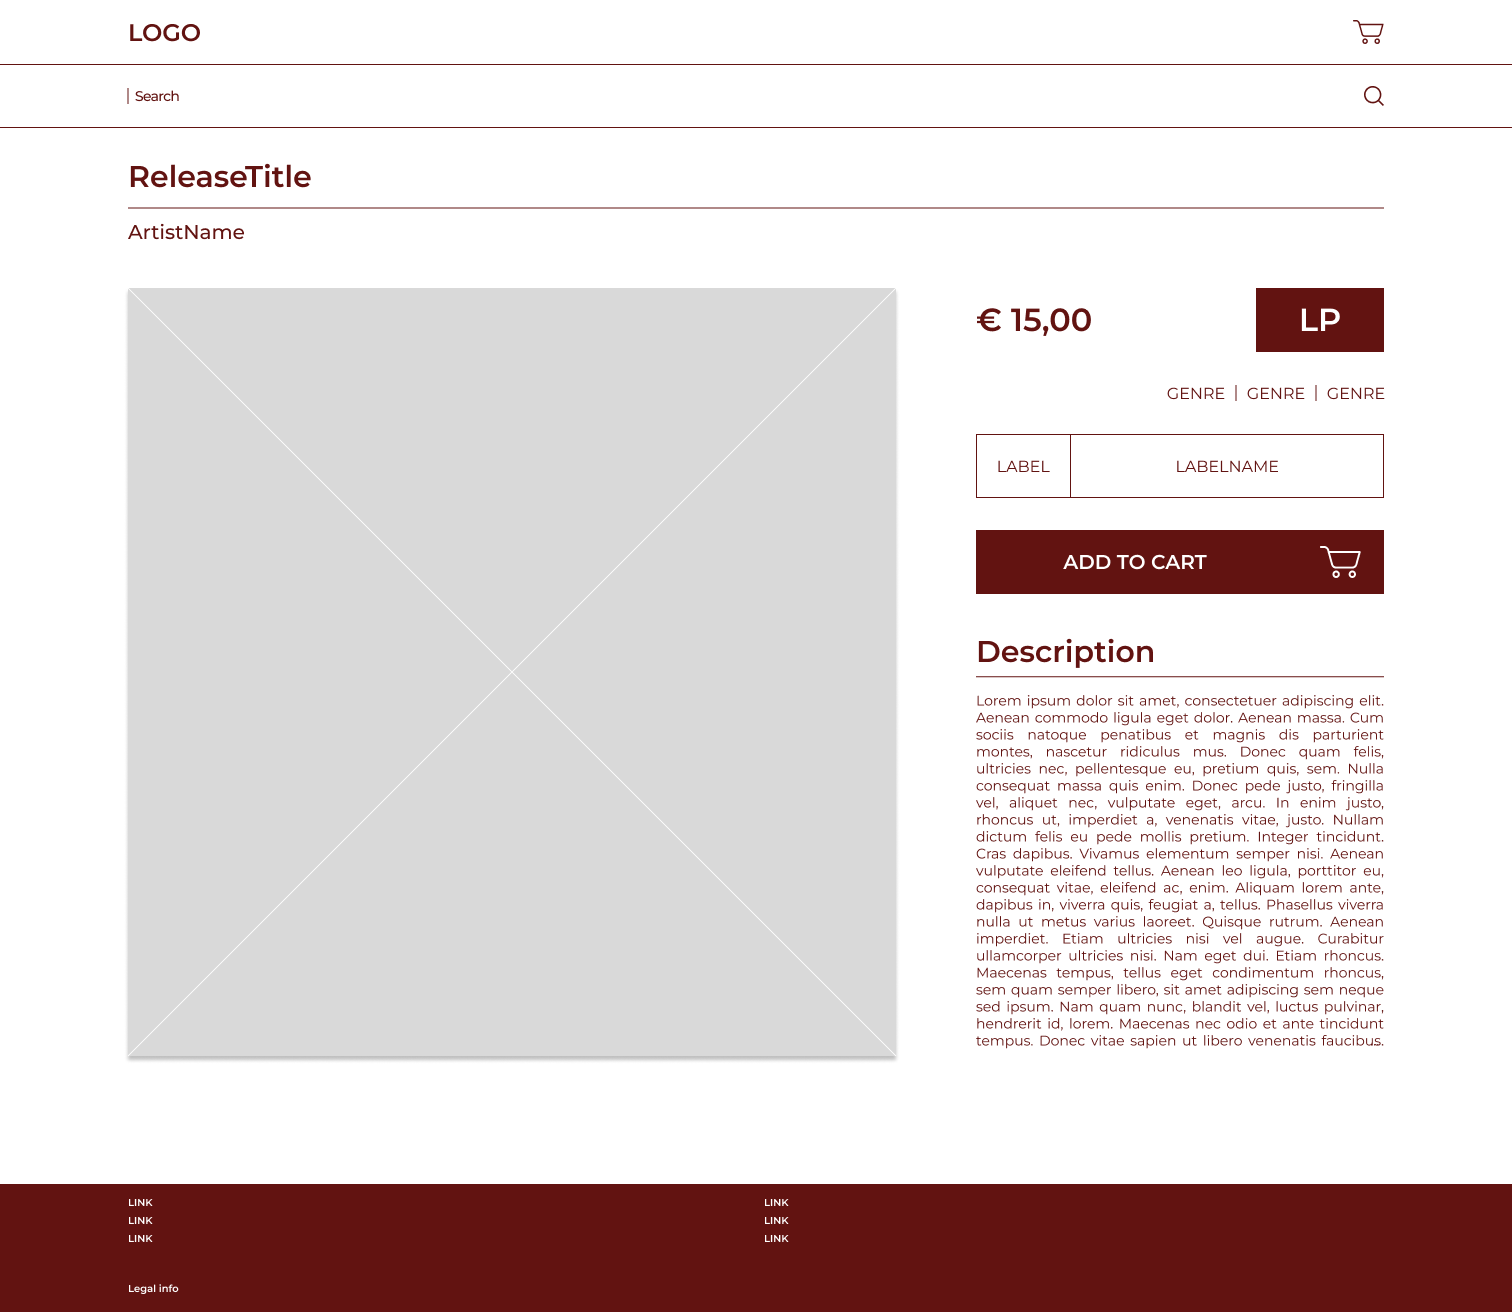
\includegraphics[width=1\linewidth]{graphics/DetailPageDesktop}
	\caption[Mock-Up Desktop]{Mock-Up Desktop Detail Pagina}
	\label{fig:desktopDetailMockUp}
\end{figure}

\pagebreak

\section{Home pagina}

\subsection{Navigeren door de home pagina}
De opbouw van de home pagina is als volgt. Wanneer men de conventionele webshop opent dan krijgt men een Trending pagina te zien, deze is gebaseerd op de nieuwste releases van Spotify. Als de gebruiker klikt op een ReleaseItem dan wordt die verwezen naar de Detail pagina van deze release. De gebruiker kan ook op "Show More" klikken indien hij/zij meer dan 8 releases wil zien. Zie figuur \ref{fig:desktopHomeConventioneel} voor een beeld van de home pagina.

\subsection{Componenten}

\subsubsection{Trending}

Deze component haalt alle nieuwste releases op a.d.h.v een provider. Hierna wordt over de releases geïtereerd en voor elke release een ReleaseItem aangemaakt.

\subsubsection{ReleaseItem}

De ReleaseItem bestaat uit de album afbeelding, de titel en de prijs van het album. De afbeelding, titel en artiesten naam worden uit de Spotify API gehaald maar de prijs is gegenereerd m.b.v. een hook genaamd useAlbumPrices die zich in de provider bevindt. Bij het initialiseren van de provider wordt deze hook aangeroepen, waarbij elke opgehaalde release een prijs krijgt toegewezen. De gegenereerde prijzen worden samen met de id van de release opgeslagen in de localStorage. Hierdoor blijven de prijzen hetzelfde en moeten ze niet telkens opnieuw gegenereerd worden.

\subsection{Hindernissen en uitdagingen}

De grootste uitdaging van de home pagina was het genereren van de prijzen voor iedere release. Hierbij zijn veel mogelijke opties overlopen bijvoorbeeld werken met een databank om de prijzen bij te houden. De reden dat geopteerd is om deze data in de localStorage op te slaan is dat hiervoor geen API calls nodig zijn.

\begin{figure}
	\centering
	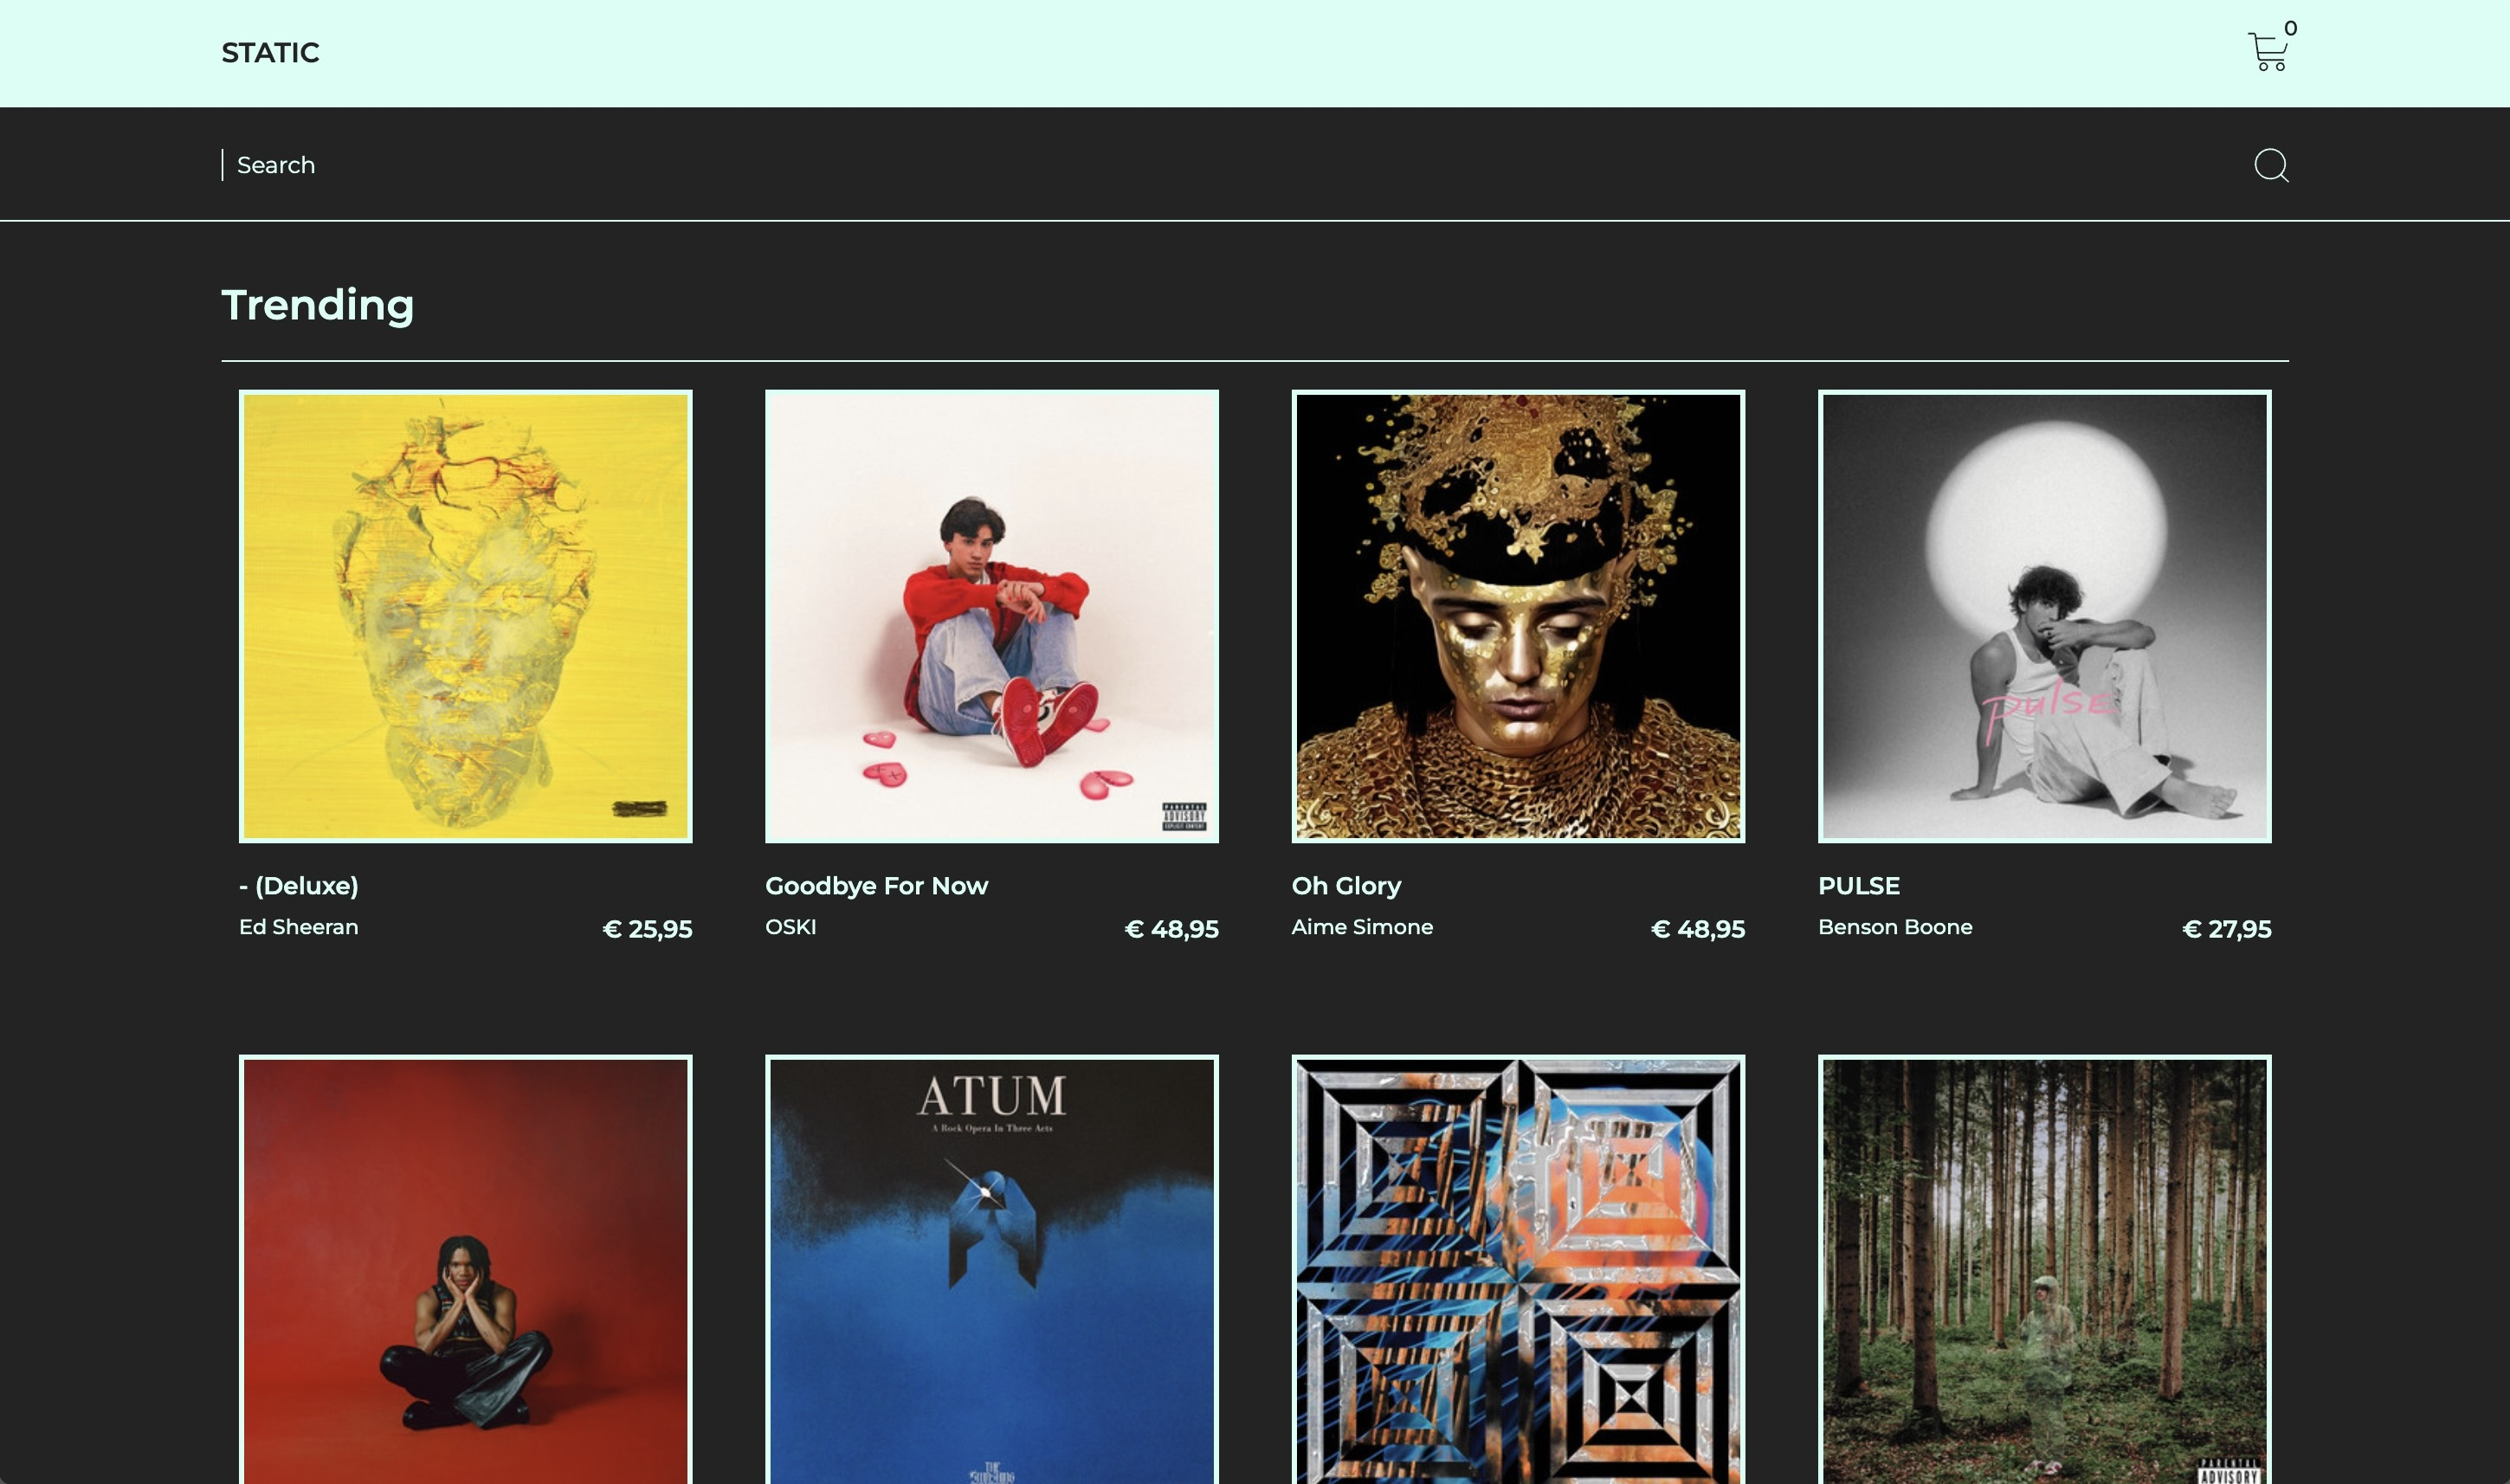
\includegraphics[width=1\linewidth]{graphics/desktopHomeConventioneel}
	\caption[Desktop home pagina conventioneel]{Desktop home pagina conventioneel}
	\label{fig:desktopHomeConventioneel}
\end{figure}

\newpage

\section{Detail pagina}

\subsection{Navigeren door de detail pagina}

Wanneer de gebruiker zich op de Detail pagina bevindt worden alle details getoond van de release. Waaronder de prijs, de releasedatum, het label en alle liedjes die behoren tot de release. De gebruiker heeft twee opties. Met de "ADD TO CART" knop kan men een release toevoegen aan de winkelmand of men kan ook doorverwezen worden naar Spotify om daar de release te beluisteren. Hier krijgt men ook opnieuw de mogelijkheid om naar een andere release te zoeken a.d.h.v. de zoekbalk. Als men een release toevoegt aan de winkelmand dan krijgt de gebruiker een pop-up ter bevestiging met twee opties, blijven door winkelen of naar de cart doorverwezen worden. Zie figuur \ref{fig:desktopDetailConventioneel} voor een beeld van de detail pagina.

\subsection{Hindernissen en uitdagingen}

Bij de detail pagina zijn weinig hindernissen opgetreden, een van de uitdagingen was om een 'GO BACK' knop te voorzien. Deze is nog op het laatste toegevoegd en vanuit een design perspectief dus niet het optimale moment. De knop bevindt zich nu in de header i.p.v. in vervanging van het logo als men naar een pagina gaat die niet de home pagina is. Wanneer een release toegevoegd wordt dan zal deze opgeslagen worden in de localStorage.

\begin{figure}
	\centering
	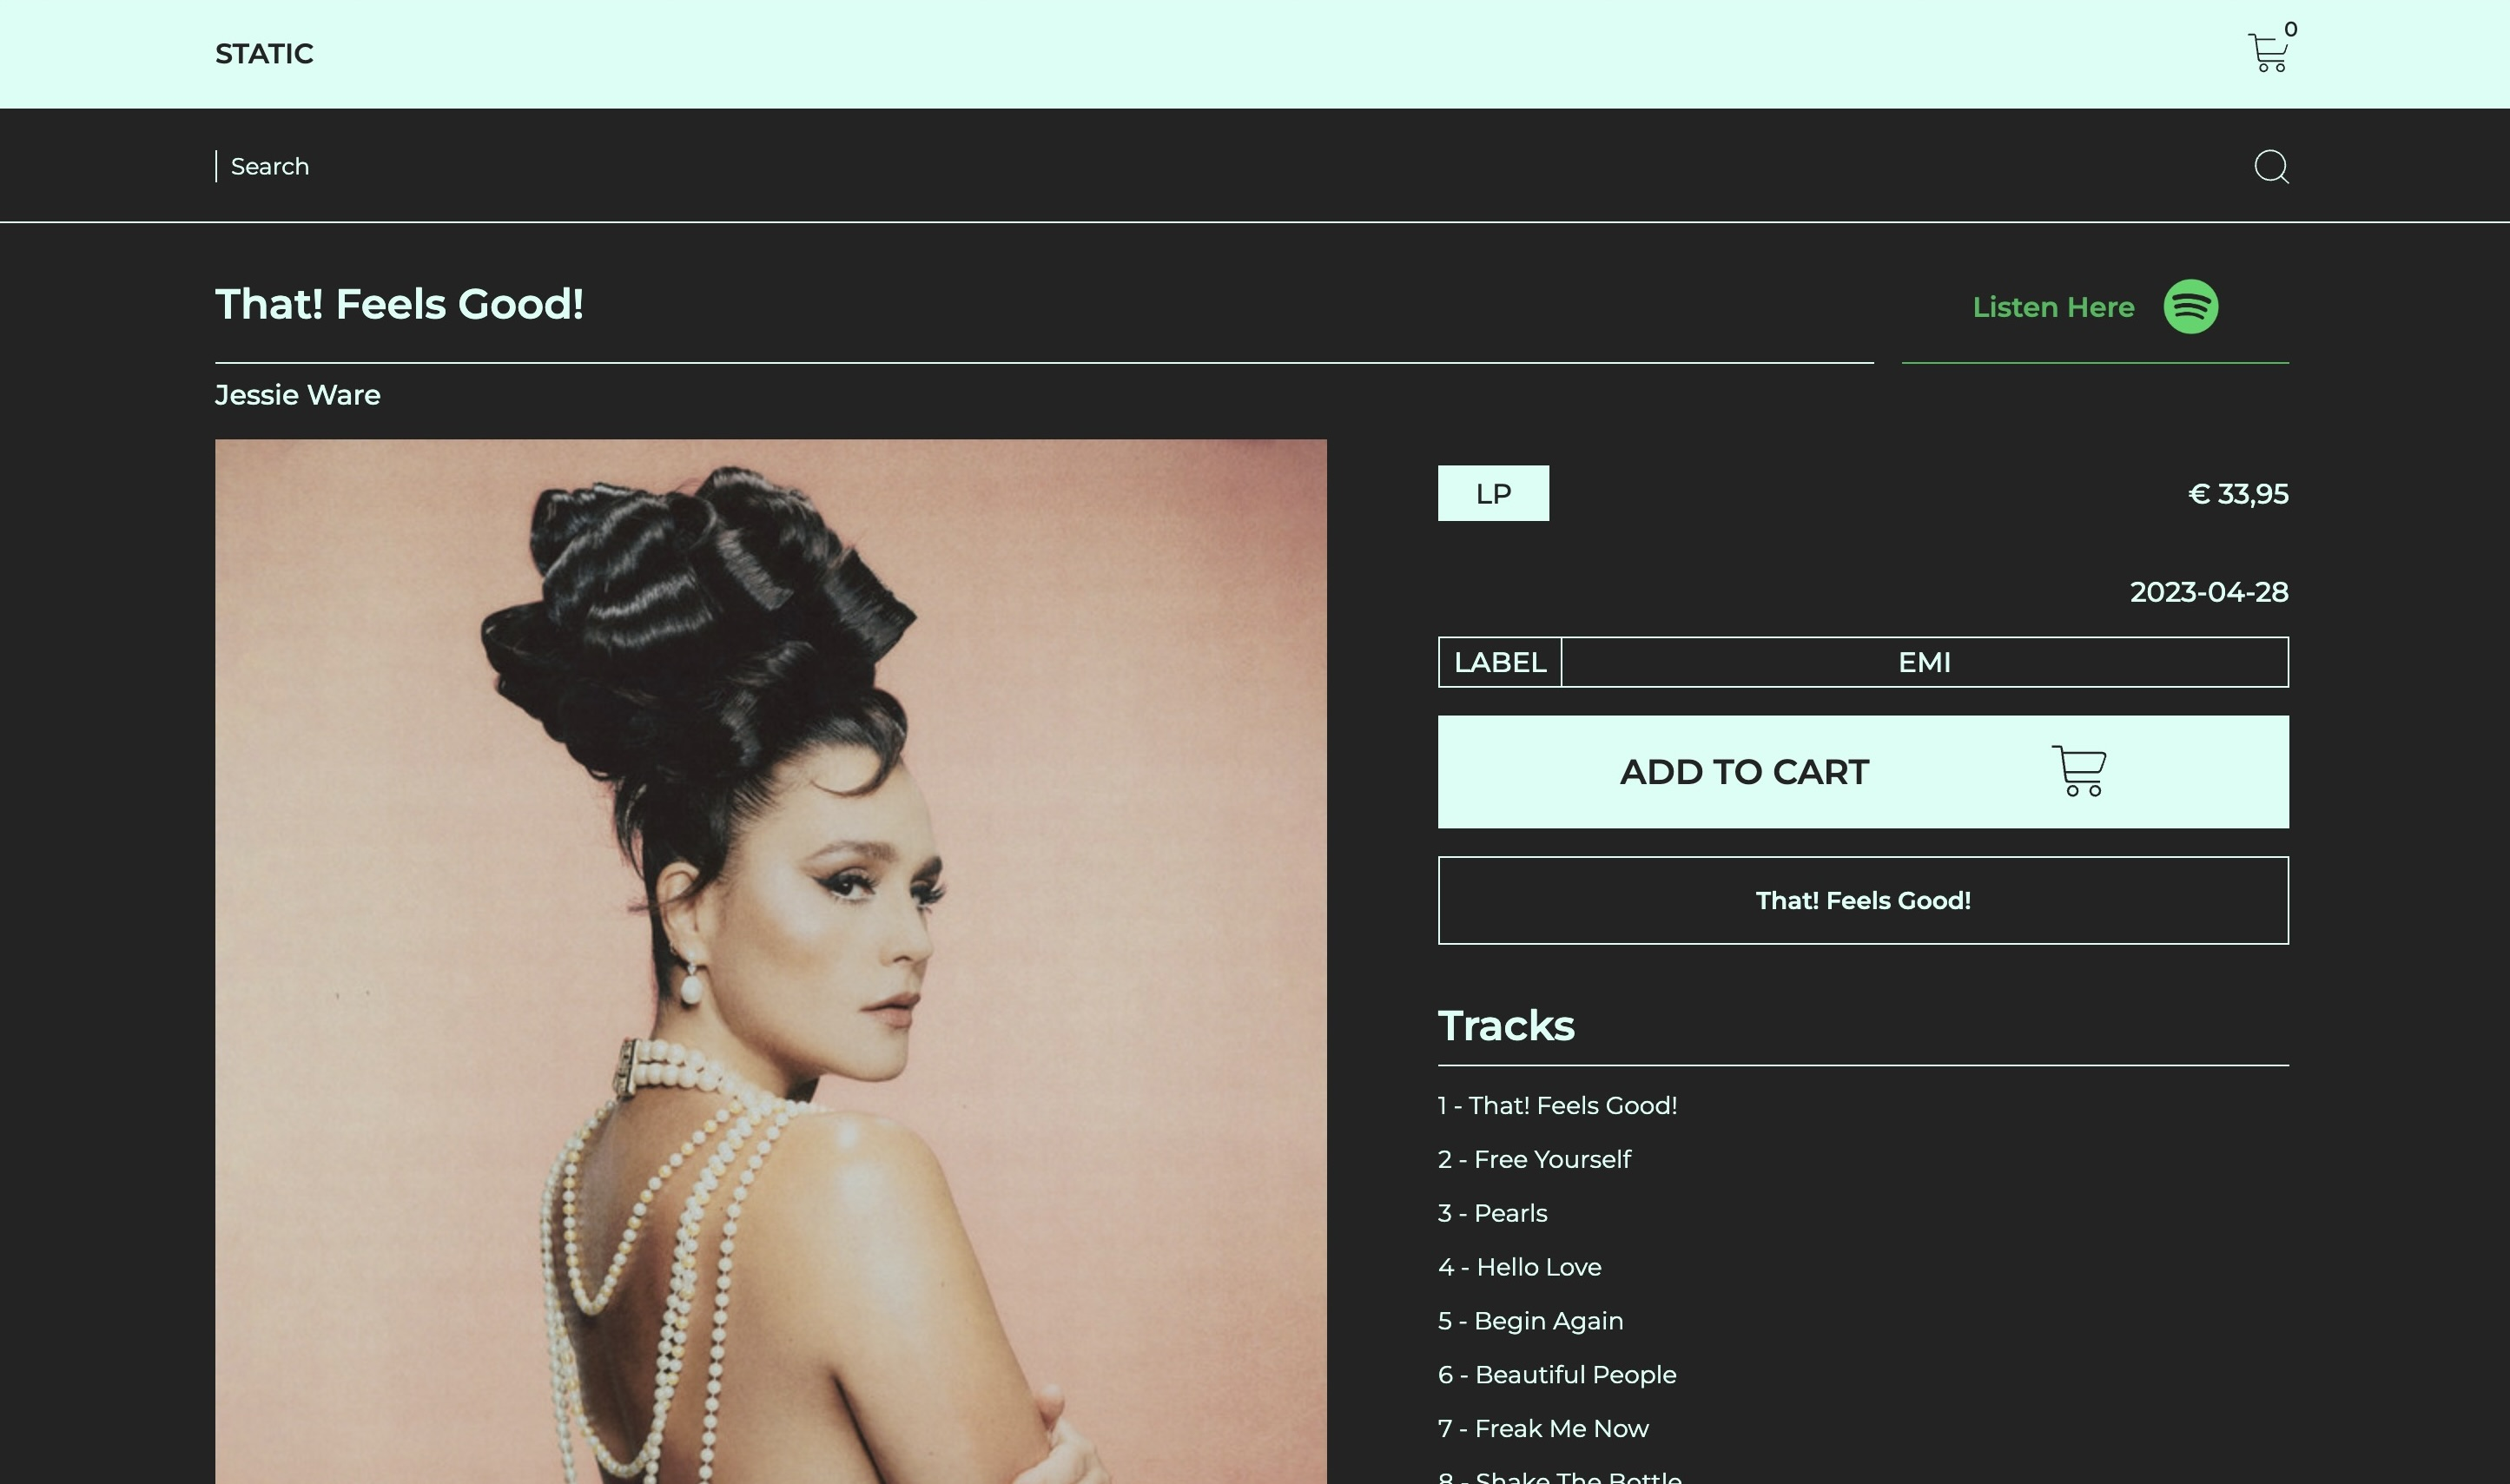
\includegraphics[width=1\linewidth]{graphics/desktopDetailConventioneel}
	\caption[Desktop detail pagina conventioneel]{Desktop detail pagina conventioneel}
	\label{fig:desktopDetailConventioneel}
\end{figure}

\section{Cart}

\subsection{Navigeren door de cart pagina}

Nu kan de gebruiker de geselecteerde releases bekijken in de winkelmand door in de header op het winkelmand icoon te klikken of bij het toevoegen aan de winkelmand op 'Go To Cart' te klikken. Hier krijgt men een overzicht van alle geselecteerde releases en kan men indien gewenst de hoeveelheid aanpassen of bepaalde releases verwijderen. Zie figuur \ref{fig:desktopCart} voor een beeld van de cart pagina.

\subsection{Componenten}

\subsubsection{Cart}

De Cart component haalt alle cartItems op uit de localStorage waar het id van de release wordt bijgehouden samen met de kwantiteit en prijs. Hierna worden een aantal calculaties uitgevoerd zijnde het berekenen van het aantal items in de cart samen met de totale prijs om de gebruiker een duidelijk overzicht te geven van de order. Voor elk item wordt een CartItem component aangemaakt en indien er geen items zijn dan word een gepaste boodschap getoond.

\subsubsection{CartItem}

Een CartItem bestaat uit de afbeelding en naam van de release, een dropdown keuzevak waarbij de kwantiteit kan veranderd worden indien gewenst, een 'Remove' knop en de individuele prijs van het item.

\begin{figure}
	\centering
	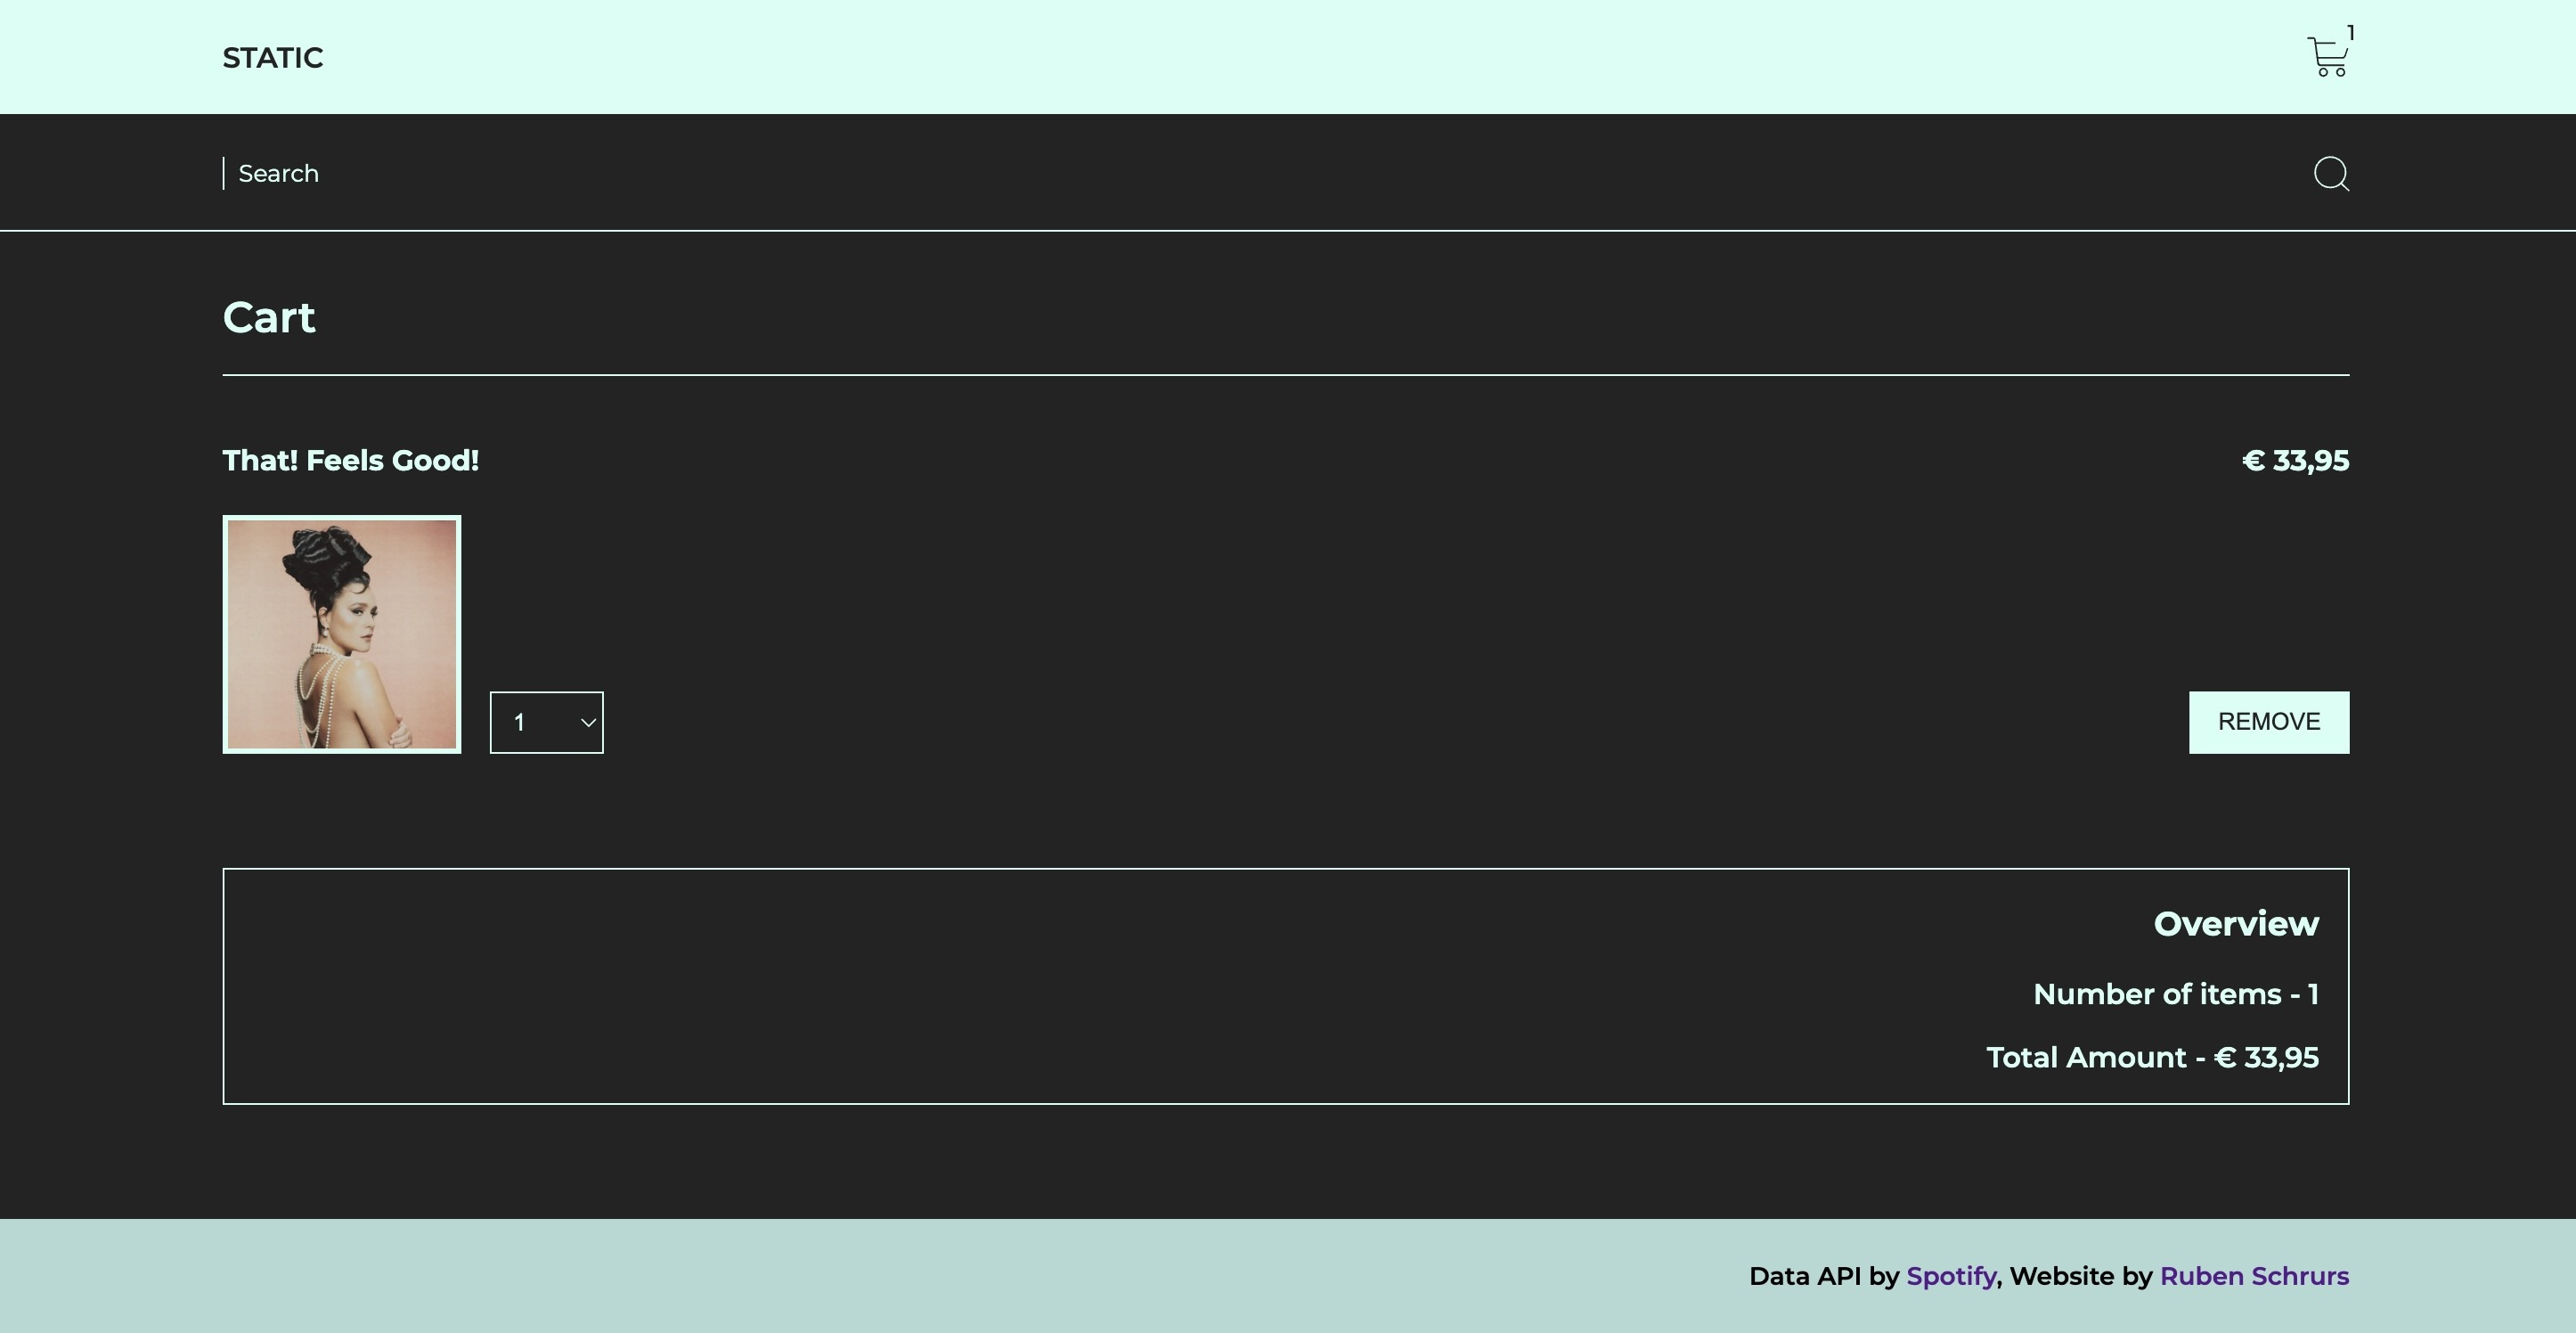
\includegraphics[width=1\linewidth]{graphics/desktopCart}
	\caption[Desktop cart pagina]{Desktop cart pagina}
	\label{fig:desktopCart}
\end{figure}

\section{Search}

Onder de header bevindt zich de search bar, deze kan de gebruiker over de volledige website gebruiken en zal volgend resultaat opleveren, zie figuur \ref{fig:desktopSearch}. De resultaten kunnen verborgen worden a.d.h.v. een 'Clear' knop rechts boven. De search bar maakt gebruik van de ReleaseItem component 

\subsection{Hindernissen en uitdagingen}

Een van de uitdagingen was om een prijs te genereren voor elk ReleaseItem wanneer de gebruiker een zoek query uitvoert. Hiernaast worden enkel resultaten getoond als er twee of meer karakters zijn in de query van de gebruiker, de reden hiervoor is om minder API calls uit te voeren.

\begin{figure}
	\centering
	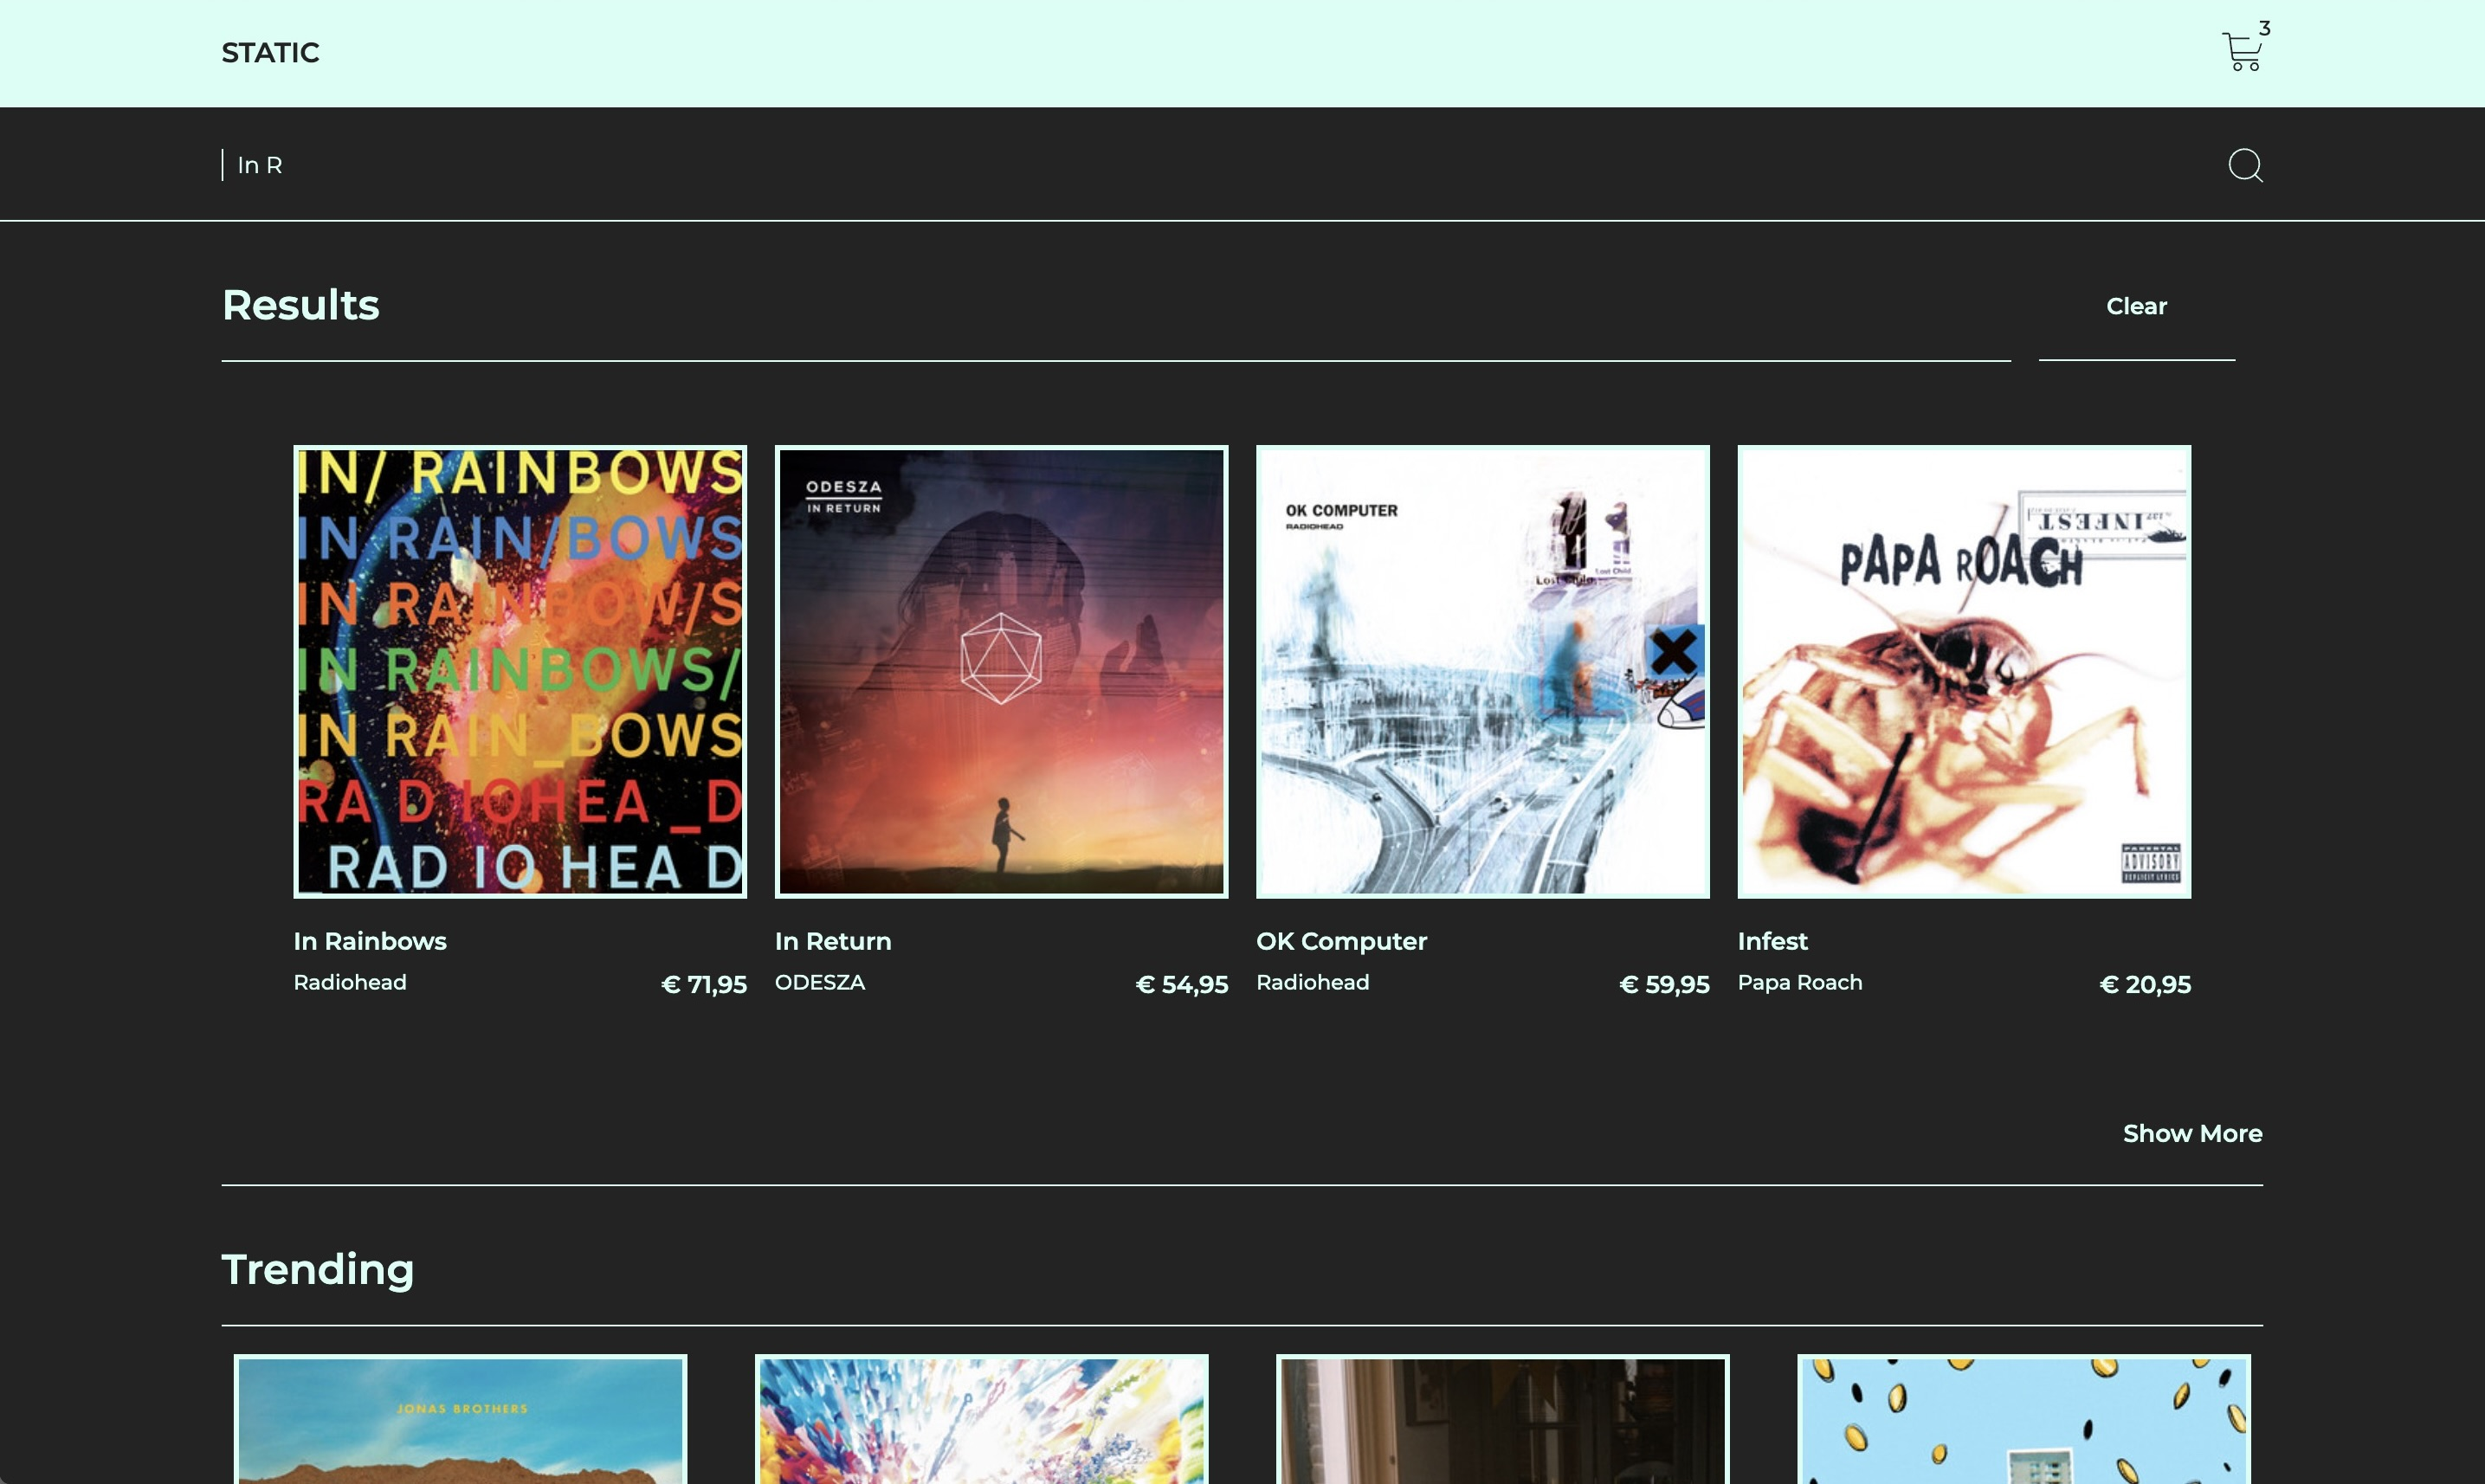
\includegraphics[width=1\linewidth]{graphics/desktopSearch}
	\caption[Desktop search]{Desktop search}
	\label{fig:desktopSearch}
\end{figure}

\section{Header}

De header bevindt zich uiteraard bovenaan en toont het logo en de cart met het aantal items in de cart. Als de gebruiker zich op de detail pagina of cart pagina bevindt dan wordt het logo vervangen door een 'GO BACK' knop.

\subsection{Hindernissen en uitdagingen}

Bij het tonen van het aantal items in de cart wordt een methode gebruikt die zich bevindt in de provider. Dit had een probleem opgelost waarbij de state van het aantal items niet geüpdatet werd ondanks er nieuwe items werden toegevoegd of de kwantiteit veranderd werd in de cart.